\documentclass[tikz,border=10pt]{standalone}
\begin{document}
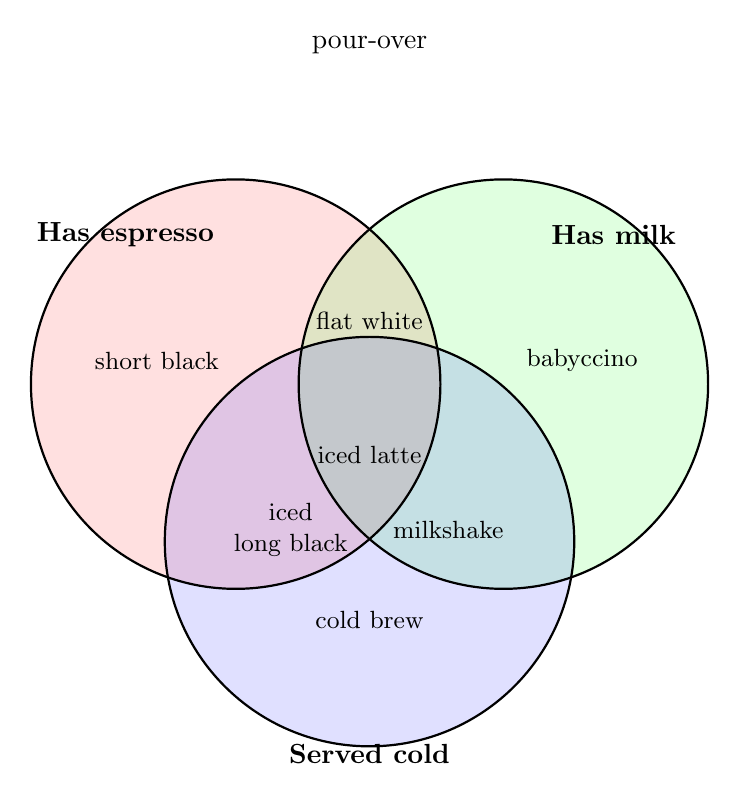
\begin{tikzpicture}[drink/.style={font=\small}]
  \def\r{2.6}
  \def\sep{1.7}
  \coordinate (A) at (-\sep,0);
  \coordinate (B) at (\sep,0);
  \coordinate (C) at (0,-2.0);
  \begin{scope}[fill opacity=0.12]
    \fill[red]   (A) circle (\r);
    \fill[green] (B) circle (\r);
    \fill[blue]  (C) circle (\r);
  \end{scope}
  \draw[thick] (A) circle (\r);
  \draw[thick] (B) circle (\r);
  \draw[thick] (C) circle (\r);

  \node[font=\bfseries] at (-3.1,1.9) {Has espresso};
  \node[font=\bfseries] at (3.1,1.9) {Has milk};
  \node[font=\bfseries] at (0,-4.7) {Served cold};

  \node[drink] at (-2.7,0.3) {short black};
  \node[drink] at (2.7,0.3) {babyccino};
  \node[drink] at (0,-3.0) {cold brew};
  \node[drink] at (0,0.8) {flat white};
  \node[drink,align=center] at (-1.0,-1.85) {iced\\long black};
  \node[drink] at (1.0,-1.85) {milkshake};
  \node[drink] at (0,-0.9) {iced latte};
  \node at (0,4.3) {pour-over};
\end{tikzpicture}
\end{document}
